%-*- coding: UTF-8 -*-
\documentclass[hpyerref,UTF8,a4paper,titlepage,12pt,oneside]{ctexbook}
\usepackage{hyperref}
\usepackage{geometry}
\usepackage{xeCJK, fontspec, xunicode, xltxtra,ulem}
\usepackage{amsthm}
\usepackage{amsmath}
\usepackage{amssymb}
\usepackage{mathrsfs}
\usepackage{mathtools}
\usepackage{commath}
\usepackage{listings}
\usepackage{float}
\usepackage{xcolor}
\usepackage{mdframed}

% \graphicspath{{../images/}}
\geometry{a4paper,bottom=2cm}

\title{流形上的矢量}
\author{陈国庆}
\date{\today}

\bibliography{plain}

% 定理结构
\theoremstyle{definition}
\newtheorem{definition}{定义}[section]
\newtheorem{theorem}{定理}[section]
\newtheorem{corollary}{推论}[theorem]
\newtheorem{lemma}[theorem]{Lemma}
\renewcommand\qedsymbol{$\blacksquare$}

\begin{document}

\maketitle
% \tableofcontents

流形上的矢量到底是什么?切矢与矢量有什么区别?一般几何书上都语焉不详,讲的不够形象,本文试图将矢量定义

\subsubsection*{矢量定义}

在$R^n$中“矢量”的意义是明确的,是有大小、有方向的“箭头”,并且与箭头的起始位置无关。\\

一般流形上没有定义“大小”、“方向”这些概念,那矢量的本质是什么呢?\\

考虑某个向量$\mathbf{v} = (v_1,v_2,v_3)$,函数$f(x,y,z)$沿$\mathbf{v}$的方向导数为,
$$
	D_\mathbf{v}(f) \equiv\nabla_f \cdot \mathbf{v}
$$

由此看出矢量$\mathbf{v}$可看作$\mathscr{F}_{\mathbb{R}^3} \mapsto \mathbb{R} $的映射,$\mathscr{F}_{\mathbb{R}^3}$是$\mathbb{R}^3\mapsto \mathbb{R}$的函数集合。\\

容易验证,$D_\mathbf{v}$是线性映射,

$$
	D_\mathbf{v}(\alpha f+ \beta g) = \alpha D_\mathbf{v}(f) + \beta D_\mathbf{v}(g)
$$

且满足莱布尼兹律,
$$
	D_\mathbf{v}(fg) = fD_\mathbf{v}(g) + gD_\mathbf{v}(f)
$$

由此可见,矢量本质是一个线性映射,推广到一般流形,定义为:\\

\textbf{流形$M$上的矢量$v$是$\mathscr{F}_M \mapsto \mathbb{R} $的,满足莱布尼兹律的线性映射。}\\

即,
\begin{equation} \label{v_linear}
	v(\alpha f+ \beta g) = \alpha v(f) + \beta v(g),\forall f,g \in \mathscr{F}_M,\forall \alpha,\beta \in \mathbb{R}
\end{equation}

及
\begin{equation} \label{v_leb}
	v(fg) = fv(g) + gv(f),\forall f,g \in \mathscr{F}_M
\end{equation}

容易验证,$v$作用在常量上为$0$。\\

大多数几何书上对矢量的定义就到此为止了,我们很难从这个定义“想象”出流形上的矢量到底长什么样子。

\subsubsection*{曲面的方向导数}

上面的定义,在通过方向导数探索矢量本质时,更注重“导数”计算过程,而忽略了“方向”的本质。\\

\begin{figure}[H]
	\begin{center}
		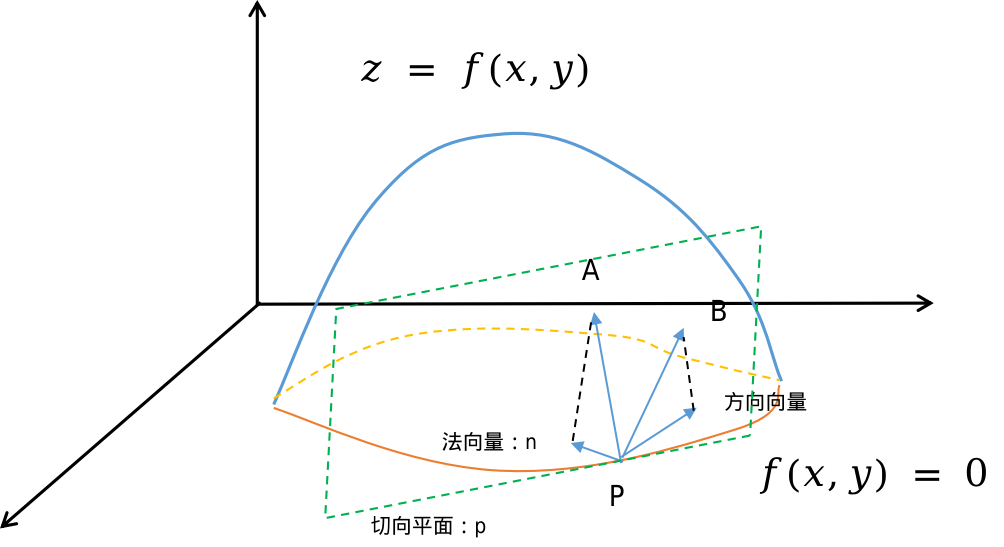
\includegraphics[width=0.8\textwidth]{images/direct_vector.png}
	\end{center}
	\caption{方向向量、方向导数、法向量、切平面}
\end{figure}	

如图所示,$z=f(x,y)$的曲面代表一座山,注意这是一个$\mathbb{R}^2 \mapsto \mathbb{R}$的映射,曲面在$P$点切面是绿色平面$p$,$P$点对应的等高面是$f(x,y) = 0$\\

可以沿着$PA,PB$两个方向(称为\textbf{方向向量})走,因为必须顺着山坡走,所以$PA,PB$都相切于曲面,也就是说$PA,PB$都位于曲面在$P$点的切面中。\\

这非常重要,这说明\textbf{曲面的方向向量是曲面切平面中的向量,即曲面的切向量。}\\

$PA$在等高面的投影是曲线$f(x,y) = 0$的法向量$n$,也是$z=f(x,y)$的\textbf{梯度向量};而$PB$在等高面的投影是一个一般向量。\\

沿着哪个方向爬会更快呢?这就是所谓方向导数的问题,方向导数反应的是沿着某个方向函数值的增量。\\

注意到,$PA,PB$只有在法向量$n$上的投影才能带来$z$的增量,在垂直于法向量的方向,函数没有定义,增量为了$0$;\\

所以,各种书上会经常指着$PA,PB$在$n$上的投影为方向向量,因为曲面的定义域是$\mathbb{R}^2$,方向向量在定义域内合情合理。\\

如此可以明确,\textbf{曲面的切向量就是方向向量(矢量),可按任意切向量计算方向导数;反之,能计算方向导数的算子就是切向量。}\\

所以,\textit{曲面上的方向向量、矢量、切向量、切矢实际都是切平面中的切向量。}

\subsubsection*{曲面曲线的方向导数}

\begin{figure}[H]
	\begin{center}
		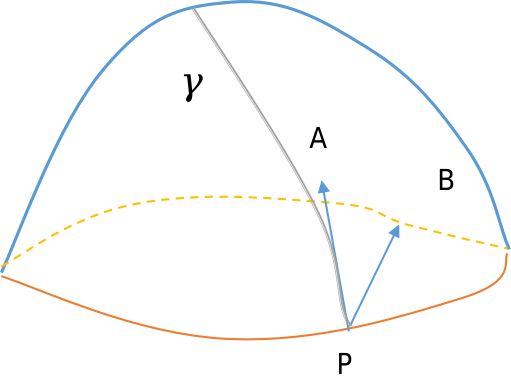
\includegraphics[width=0.8\textwidth]{images/vector2.png}
	\end{center}
\end{figure}	

现在把坐标系拿掉,我们应该知道$PA,PB$依然处在$P$点的切平面中,考虑曲面上灰色的曲线$\gamma$,其与切平面相切;\\

$PA$是曲线$\gamma$的切向量,$PB$是一般方向,沿$PB$方向,$\gamma$的增量是多少呢?\\

实际还是方向导数问题,增量大小依赖$PB$在$PA$的投影长度。\\

曲线是定义在曲面上的函数,曲线的方向向量就只能是向量$PA,PB$,这样曲面上的方向向量终于跟曲面有了直接的关系。\\

这说明:\textit{定义在曲面上曲线的方向向量,就是曲面的切向量本身。}\\

曲面是定义在$\mathbb{R}^2$的函数,可以说$PA,PB$在$n$的投影向量是方向向量,看出其区别了吗?

\begin{itemize}
\item 定义在$\mathbb{R}^2$上的曲面的方向向量属于$\mathbb{R}^2$,定义域与切空间一致
\item 定义在曲面上的曲线的方向向量不再属于曲面,定义域与切空间不一致
\end{itemize}

这种不一致说明,曲面作为一个流形,与$\mathbb{R}^n$空间有本质区别。\\

或者说,$\mathbb{R}^n$空间中某个点的切空间还是$\mathbb{R}^n$,但对一般流形不成立。

\subsubsection*{流形上的矢量}

我们还有两个观察:

\begin{enumerate}
	\item 一元函数的切空间是一条直线($\mathbb{R}^1$),二元函数的切空间是一个平面($\mathbb{R}^2$),可验证,$n$元函数切空间是$\mathbb{R}^n$
	\item 过曲线一点只能有一个切向量与之对应,但一个切向量可以对应多条曲线,所以有些书上也会把向量用曲线的等价类来定义
\end{enumerate}

基于上述两个观察,对比曲面,流形上well-defined的矢量需满足,
\begin{itemize}
	\item 流量上的矢量空间不应与流形一致
	\item 流形上的矢量反映到二维曲面上,应是曲面的切向量
	\item 流形上的矢量是多条定义在流形上曲线的切线
	\item $n$维流形的矢量空间应该线性同构于$\mathbb{R}^n$
\end{itemize}

实际上只要我们证明了最后一条同构,前两条自然也就成立了;而曲线切向量这个是需要我们给出定义去验证的。

\subsubsection*{切空间}

	流形$M$在$p$点的切空间记为$V_p$,根据定义是一些满足(\ref{v_linear}),(\ref{v_leb})的算子,需定义数乘和加法来构成线性空间,
	$$
		v(\alpha f) = \alpha v(f), \forall v \in V_p
	$$

	$$
		(v + \nu )f = v(f) +\nu(f), \forall v,\nu \in V_p 
	$$

	接下来需证明$\mathbb{R}^n$与$V_p$线性同构。首先构造一个从$\mathbb{R}^n\mapsto V_p$的映射,
	$$
		D_v :v \mapsto \sum_{i=1}^nv^i\frac{\partial f}{\partial x^i}\Big|_{x_p} = \nabla f_{x_p} \cdot v
	$$

	这里讨论的是$p$点的切空间,所以存在坐标卡$(U,\phi)$,$f$实际是指$f\circ \phi^{-1}$,是$\mathbb{R}^n \mapsto \mathbb{R}$的映射,并且$\phi(p) = x_p$\\

	显然$D_v$满足(\ref{v_linear}),(\ref{v_leb}),是一个矢量。\\

	 \textbf{(i) $D_v$是一个单射},对$\forall \nu \in \mathbb{R}^n, \forall f \in \mathscr{F}_M$
	$$
		D_v = D_\nu \Rightarrow \nabla f_p \cdot (v - \nu) = 0 \Rightarrow v = \nu
	$$

	\textbf{(ii) $D_v$是满射},$\forall f \in \mathscr{F}_M$,作一阶泰勒展开
	$$
		f(x) = f(x_p) + \sum_{i=1}^n(x^i - x_p^i)\frac{\partial{f}}{\partial{x^i}}\Big|_{x_p}
	$$

	对$\forall D \in V_p$,作用在上式两边,根据线性性及莱布尼兹律,
	$$
		D(f) = D(f({x_p})) 
			+ \sum_{i=1}^nD\left(x^i - x_p^i\right)\frac{\partial{f}}{\partial{x^i}}\Big|_{x_p} 
			+ \sum_{i=1}^n(x^i - x_p^i)D\left(\frac{\partial{f}}{\partial{x^i}}\Big|_{x_p}\right)
	$$

	注意,$x_p,f(x_p),\frac{\partial{f}}{{\partial x^i}}|_{x_p}$,均为常量,所以作用$D$后为$0$,
	$$
		D(f) = \sum_{i=1}^nD\left(x^i\right)\frac{\partial{f}}{\partial{x^i}}\Big|_{x_p} = \nabla_{f(x_p)} \cdot v
	$$

	其中$v = (D(x^1),\dots,D(x^n))$,根据定义是一个$n$维向量。\\

	\textbf{(iii) $D_v$保线性结构}
	$$
		D_{v + \nu}(f) = \nabla f_{x_p} \cdot (v + \nu) = \nabla f_{x_p} \cdot v + \nabla f_{x_p} \cdot \mathbf{\nu} = D_v(f) + D_{\nu}(f)
	$$

	$V_p$与$\mathbb{R}^n$的线性同构得到证明。

\subsubsection*{流形上的曲线}
	曲线实际就是一些点的集合,所以常用$I \mapsto M$的映射来表示一条曲线($I$是$\mathbb{R}$的闭区间),如果流形$M$退化到一个圆,就是$[0,2\pi]\mapsto \mathbb{R}$的映射,
	$$
		C: t \mapsto (\cos t,\sin t), t\in [0,2\pi]
	$$

	这实际就是曲线的参数方程,参数方程的梯度便是曲线的切向量,比如圆的切向量为$C^\prime(t) = (-\sin t,\cos t)$。\\

	如果一条曲线的定义域$I = \mathbb{R}$则称为\textbf{完备曲线}。

\subsubsection*{曲线切矢量}
	$C(t)$是流形$M$上的$C^1$曲线,则$C(t_0)$点的切矢量定义为下面的映射,
	$$
		T(f) \equiv \frac{d(f\circ C)}{dt}\Big|_{t_0},\forall f \in \mathscr{F}_{M}
	$$

	注意,这里的$f$就是定义本身。在不引起歧义的情况下也可记作,
	$$
		T(f) \equiv \frac{df}{dt}\Big|_{t_0}
	$$

	此时$f$是$f\circ C$复合函数,是$I\mapsto \mathbb{R}$的映射。

	\begin{figure}[H]
		\begin{center}
			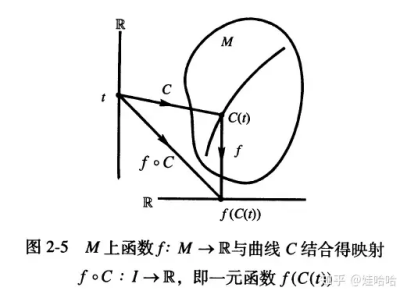
\includegraphics[width=0.8\textwidth]{images/curve.png}
		\end{center}
	\end{figure}

	$$
		T(f) = \frac{d(f\circ C)}{dt} = \frac{df}{dC}C^\prime(t) = \nabla f\cdot C^\prime\Big |_t
	$$

	又出现了这个熟悉的形式。\\

	曲线的参数表示式的梯度$C^\prime(t)$为曲线的切向量,所以$T(f)$的结果可解释为,沿着曲线切向量$C^\prime(t)$计算$f$的方向导数,根据定义,$T$显然是一个矢量,并且是$C(t)$的切矢量。\\


	至此,流形上的矢量已经完全well-defined。\\

	\textit{再强调下,流形上的矢量、向量、切矢量、切向量都是一回事,都是指流形切空间中的矢量;而曲线的切矢量,或切向量,不能称呼为曲线的矢量或向量。}
\bibliography{math}
\end{document}